%%%%%%%%%%%%%%%%%%%%%%%%%%%%%%%%%%%%%%%%%%%%%%%%%%%%%%%%%%%%%%%%%%%%%%%%%%%%%%%%
% Event_Reconstruction_Chapter.tex:
%%%%%%%%%%%%%%%%%%%%%%%%%%%%%%%%%%%%%%%%%%%%%%%%%%%%%%%%%%%%%%%%%%%%%%%%%%%%%%%%
\chapter{Event Reconstruction}
%%%%%%%%%%%%%%%%%%%%%%%%%%%%%%%%%%%%%%%%%%%%%%%%%%%%%%%%%%%%%%%%%%%%%%%%%%%%%%%
\section{Event Reconstruction Overview}
Event reconstruction is the process of reconstructing particles and their four momenta using raw data read from the electronics of the different CMS subdetectors. Event reconstruction is archived in CMS  using the \textit{Particle Flow}~(PF) algorithm which reconstructs all the particles in an event, individually, using information from all CMS subdetectors. It is also possible to reconstruct particles without using the PF algorithm.%For example, in the calorimeter subdetectors, an energy clustering algorithm is used to produced energy clusters and in the tracker and muon chambers, a combination of tracking algorithms is used to construct particle tracks. By matching selected tracks to energy clusters, particles like photons, electrons, muons, jets and missing transverse energy~(\MET) are reconstructed.

%%%%%%%%%%%%%%%%%%%%%%%%%%%%%%%%%%%%%%%%%%%%%%
\section{Supercluster Reconstruction}
A clustering algorithm groups energy deposits from individual crystals to form clusters which are eventually grouped together forming  clusters of clusters known as \textit{superclusters}. A cluster is either a $3\times3$ or $5\times5$ crystals energy matrix. About 94\%~(97\%) of the incident photon or electron energy is deposited in the $3\times3$~($5\times5$) crystal matrix in $(\eta, \phi)$ directions in the barrel and $(x,y)$ directions in the endcaps. 
\newline
The $3.8$~T magnetic field and material in front of the calorimeter causes electrons and photons radiating off electrons to deposit their energy in a cluster of crystals spread in $\phi$ and because of the spread in $\phi$,  the clustering algorithms starts building clusters with a seed crystal~(crystal with the maximum energy) and continues within a narrow window in $\eta$ by summing the crystal energies along $\phi$, which is the direction of the energy spread due to the magnetic field. Figure \ref{fig:CLUSTER} is a schematic picture showing the direction~(left Figure) of the clustering process in $(\eta,\phi)$ directions in the barrel  and the fraction~(right Figure) of electromagnetic energy in a typical cluster.

\vspace{5mm}
\begin{minipage}{0.94\textwidth}
\begin{center}
%\begin{figure}
\mbox{
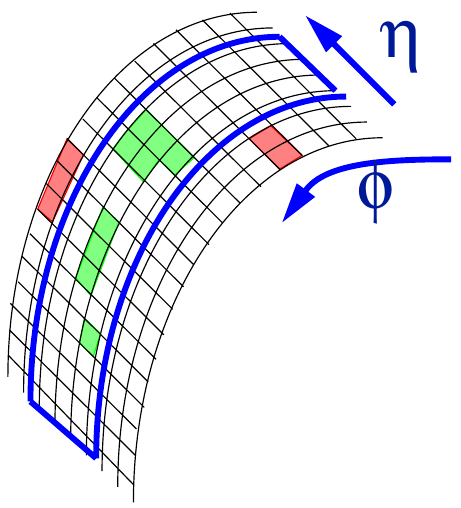
\includegraphics[height=0.35\textwidth, width=0.45\textwidth]{THESISPLOTS/ECAL_CLustering.png}\quad
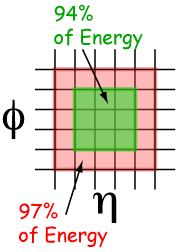
\includegraphics[height=0.35\textwidth, width=0.45\textwidth]{THESISPLOTS/BasicCluster.png}}
\captionof{figure}{Superclustering algorithm direction~(left) in the $(\eta,\phi)$ plane in EB and fraction~(right) of electromagnetic shower energy coverage in a crystal energy matrix.} 
\label{fig:CLUSTER}
%\end{figure}
\end{center}
\end{minipage}
\vspace{5mm}

Two major clustering algorithms are used in ECAL: the \textit{hybrid}~(EB) and \textit{island}~(EE) algorithms.
\begin{itemize}
\item \textbf{Hybrid Supercluster Algorithm:} This algorithm is used for making super clusters in the barrel~(EB). It takes advantage of the $\eta - \phi$ geometry of barrel crystals by taking a fixed 3 or 5 crystals in $\eta$ and dynamically search and sum separate crystals energy along $\phi$. The Hybrid algorithm takes advantage of the knowledge of the lateral shower shape along the $\eta$ direction. The supercluster consists of basic clusters which are usually $3\times3$ crystals energy matrix.
%%The figure \ref{fig:HYBRID} shows an example of how the hybrid clustering algorithm performs clustering.
%%\begin{center}
%\begin{figure}
%%\centering
%%\mbox{
%%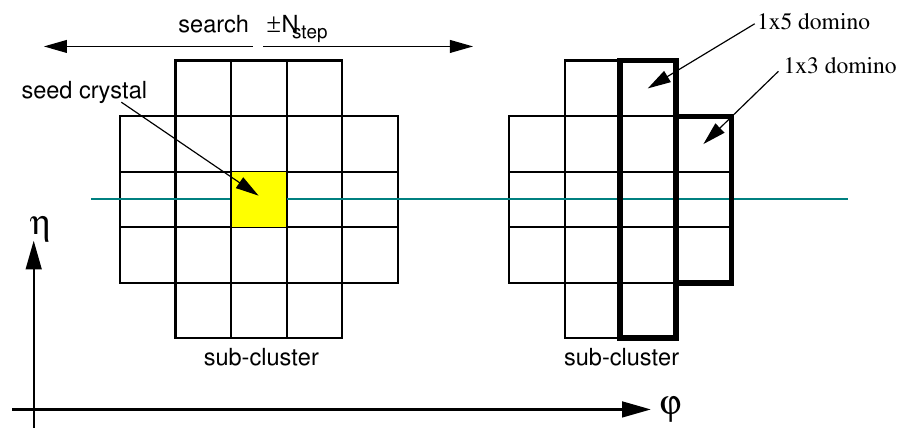
\includegraphics[height=0.35\textwidth, width=0.45\textwidth]{THESISPLOTS/Hybrid_Clustering_ECAL.png}}
%%\captionof{figure}{Superclustering in ECAL for hybrid clustering algorithm in barrel.} 
%%\label{fig:HYBRID}
%\end{figure}
%%\end{center}

\item \textbf{Island Supercluster Algorithm:} This algorithm is used for making clusters in the endcap~(EE). It begins by finding the seed crystal of the electromagnetic shower with maximum energy above a certain energy threshold. Using the seed crystal position, adjacent crystals are examined %starting fist along $\phi$ and then along $\eta$
and added to a cluster until a rise in energy where a crystal belonging to another cluster or crystal that has\ no energy hit is reached. For each crystal to be added to the cluster, its energy read must be positive, it must not have been assigned to another cluster and the previous crystal added in the same direction must have a higher energy. These non-overlapping clusters~(usually a $5\times5$ crystals energy matrix) finally form a supercluster.
%% A search is performed for the most energetic cluster and then collect all the other narrow window clusters in $\eta$ and wide window in $\phi$. The figure in \ref{fig:ISLAND} provides a pictorial view of how the island algorithm works.
%%\begin{center}
%\begin{figure}
%%\centering
%%\mbox{
%%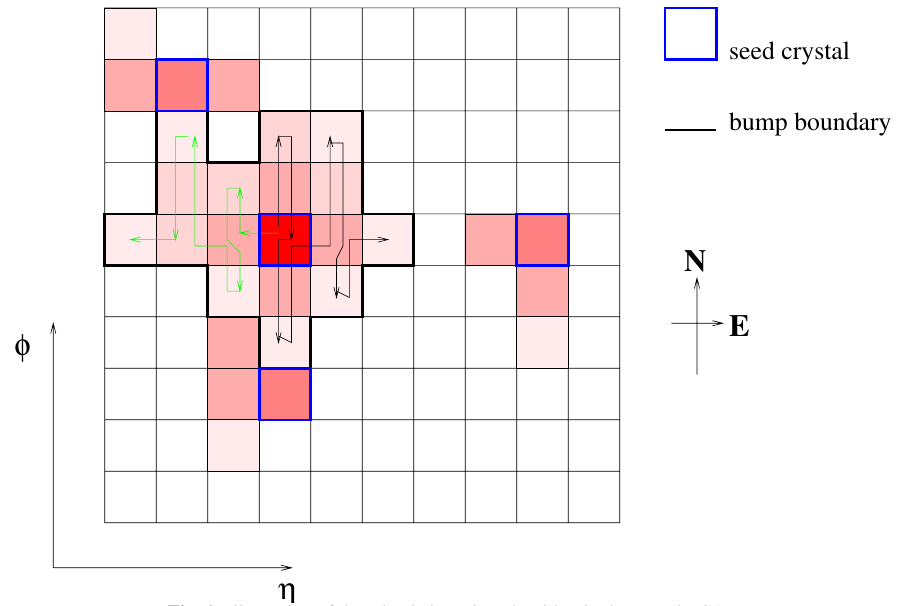
\includegraphics[height=0.35\textwidth, width=0.65\textwidth]{/home/tensr/Documents/TEN-HEP-PHD-THESIS/PHD_THESIS/PHD/THESISPLOTS/ISLAND_Clustering_ECAL.png}
%%}
%%\captionof{figure}{Superclustering using the Island clustering algorithm in barrel.} \label{fig:ISLAND}
%\end{figure}
%%\end{center}
\end{itemize} 

\section{Track and Vertex Reconstruction}
The track of a charge particle is reconstructed using \textit{hits} which are themselves reconstructed from the ionization left in silicon by the passage of the charge particle. The particle's helical trajectory or track, reconstructed from these hits, is used to measure the it's momentum and direction.
\newline
Track reconstruction uses several algorithms with the main algorithm used for reconstructing the tracks of charge particles produced from $pp$ collisions called the \textit{Combinatorial Track Finder}~(CTF). The CTF integrates track fitting and pattern recognition, building tracks from an initial trajectory or seed while taking into account the energy loss and multiple-scattering between the tracker detector layers. It proceeds in three stages: seeding, finding and fitting.
\newline
During the seeding, initial trajectories~(seeds) made of a pair of pixel hits that are compatible with the beam spot and have a lower \pt limit are used as possible candidates of the charge tracks. Pixel hits are the best track seeds while in the more forward region of the tracker detector, $2 <|\eta| < 2.5$, silicon pixel and inner strips hits are used for better track seeding.
\newline
The track finding stage uses a \textit{Kalman Filter} pattern recognition approach~(since the tracks can be described as a discrete dynamic \textit{track state}, characterized by some given set of parameters and uncertainties, which is recursively updated one hit at a time on each layer) where, starting with the track parameters determined by the seeds, the track trajectory is extrapolated to outer neighboring tracker layers and compatible hits are assigned to the track. 
\newline
In the fitting stage, the Kalman Filter algorithm~(because the position information of the hit is updated to estimate the track parameters and uncertainties and the fitting process is repetitive) is again applied  where each candidate track is fitted using least-squares fitting in two stages. The first stage avoids possible bias on the track parameters from the initial trajectories used in the seeding stage while the next stage yields the best estimates of the track parameters and uncertainties at the original vertex.
\newline
Other algorithms like the \textit{iterative tracking algorithm} which is a general purpose tracking algorithm is used in association with customized CTF tracking algorithm to reconstruct the tracks of non-collisions  events like cosmic and beam halo.
\par 
Similar to track reconstruction, vertex reconstruction involves two stages: vertex finding and vertex fitting. During vertex finding, a set of valid tracks from track reconstruction, represented by a list of track parameter vectors, is fed into a vertex finding algorithm which classifies the tracks into vertex candidates. The type of vertex finding algorithm used depends on whether it is finding a primary vertex~(vertex where the particles are produced from the collision of the two proton beams) or secondary vertex~(vertex where the particles are produced from the decay of an unstable particle) or the reconstruction of an exclusive particle decay. 
\newline
The classified vertex candidates from vertex finding are fed into the vertex fitting algorithm. The output of the vertex fitting is a list of vertices, with each vertex having an estimated vertex position and a set of updated track parameter vectors. In vertex fitting, the best estimates of the vertex parameter, co-variance matrix, track parameter and the fit quality (chi-square, number of degrees of freedom, track weights) are used in distinguishing among a given set of tracks and their vertices.

%%%%%%%%%%%%%%%%%%%%%%%%%%%%%%%%%%%%%%%%%%%%%%%%%%%%%%%%%%%%%%%%%%%%
\section{Photon and Electron Reconstruction}
\par 
Photons are reconstructed using superclusters and since they are neutral and do not leave tracks in the tracker, they are identified as superclusters in ECAL not associated to any tracks or reconstructed hits in the pixel tracker. The photon identification, beyond simply using the ECAL supercluster, is improved through several selection requirements using information from the tracker, ECAL, HCAL and the ratio of the photon candidate's energy deposited in HCAL to ECAL. Photons are supposed to deposit very little or no energy in HCAL and this is one of the main selection requirements to help distinguish photons from hadronic jets with high electromagnetic energy fraction which can easily be misidentified as photons.% and $R_{9}$, which is the ratio of the electromagnetic energy contained in a $3\times3$ matrix to the supercluster energy. 
%The $R_{9}$ variable is very useful in separating photons from the decay of \Ppizero with isolated photons since the photons from \Ppizero decay have a lower value of $R_{9}$ compared to isolated photons.
\par 
For electron reconstruction, electron candidates are found when a supercluster is associated to a track  reconstructed in the silicon tracker detector and in particular, its inner most layers~(pixel hits). Electron reconstruction begins with a seeding  approach which is either driven by ECAL or by the tracker. The ECAL driven seeding approach is very efficient for  electrons with $\pt > 10\GeVc$. The track driven seeding approach uses a boosted decision tree to perform a pre-selection of the tracker clusters, in order to reduce fake electrons which are light hadrons with many hits in the tracker. Low-\pt electrons and non-isolated electrons~(electrons embedded in jets) are reconstructed efficiently using the tracker driven seeded approach, since most of their energy is deposited in the tracker and very little in the ECAL, as they lose most of their energy through multiple scattering before they reach ECAL. When fitting the electron tracks, we must account for the different energy loss mechanisms  of the electron compared to other charged particles. Since electrons lose most of their energy by radiating photons~(\textit{bremsstrahlung}, which is non-Gaussian in nature, the \textit{Gaussian Sum Filter} algorithm~(combination of several Gaussians) is used to provide  good estimate of the track momentum both at the ECAL surface  and at the interaction point. 
%%%%%% Why Am I talking about these energy corrections?%%%%%%%%%%%%%%%%%%%%%%%%%%%%%%%%%%%
%\par 
%During $pp$ collisions, events produced from low energy $pp$ collisions called \textit{minimum bias events}, events from multiple proton-proton interactions called \textit{Pile Up}~(PU) events, poor detector calibration, poor supercluster or track reconstruction, faulty electronics and crystal transparency loss due to the high dose of radiation lead to photon or electron energy mismeasurements. Thus, the best estimate of the photon or electron's energy must include corrections for these contributions.
%\newline
%An estimate of the energy deposited by an electromagnetic particle in the ECAL, $E_{e/\gamma}$, can be approximated using Equation \ref{eq:eEnergy}; 
%\begin{equation}\label{eq:eEnergy}
%E_{e/\gamma} = F_{e/\gamma} \cdot [ G \cdot \sum_{i} S_{i}(t) \cdot C_{i} \cdot A_{i} ],
%\end{equation}
%where $A_{i}$ is the signal amplitude in ADC counts, $C_{i}$ is the inter-calibration coefficient,  $S_{i}(t)$ is the time-dependent corrections  for response variations, usually obtained from laser-based calibration, $G$ is the global scale calibration allowing to go from energy in ADC counts to \GeV and $F_{e/\gamma}$ is the particle energy corrections for geometric, clustering and other effects. The sum is over all the crystals belonging to the photon or electron supercluster. The true electron or photon energy is measured after making energy adjustments which depend on $\eta$ through $F_{e/\gamma}$ during the supercluster reconstruction to account for detector energy biases caused by cracks between crystals and in general energy containment within clusters and electronic noise. In Figure \ref{fig:EnergyCorr}, we show comparisons between cases where no energy adjustments were made to those where energy adjustments~(in the form of crystal inter-calibration and laser monitoring corrections for crystal transparency loss) have been made, through measuring the mass of the $\PZ$ boson. We see improvements on measuring the $\PZ$ mass, $91$\GeVcc, after the inter-calibration~(IC) and laser monitoring~(LM) corrections were made. Figure \ref{fig:SCEnergyCorr}, shows the case where adjustments are made during supercluster reconstruction. Once again the \PZ mass is well reconstructed after introducing these corrections.

%\vspace{5mm}
%\begin{minipage}{0.94\textwidth}
%\begin{center}
%\mbox{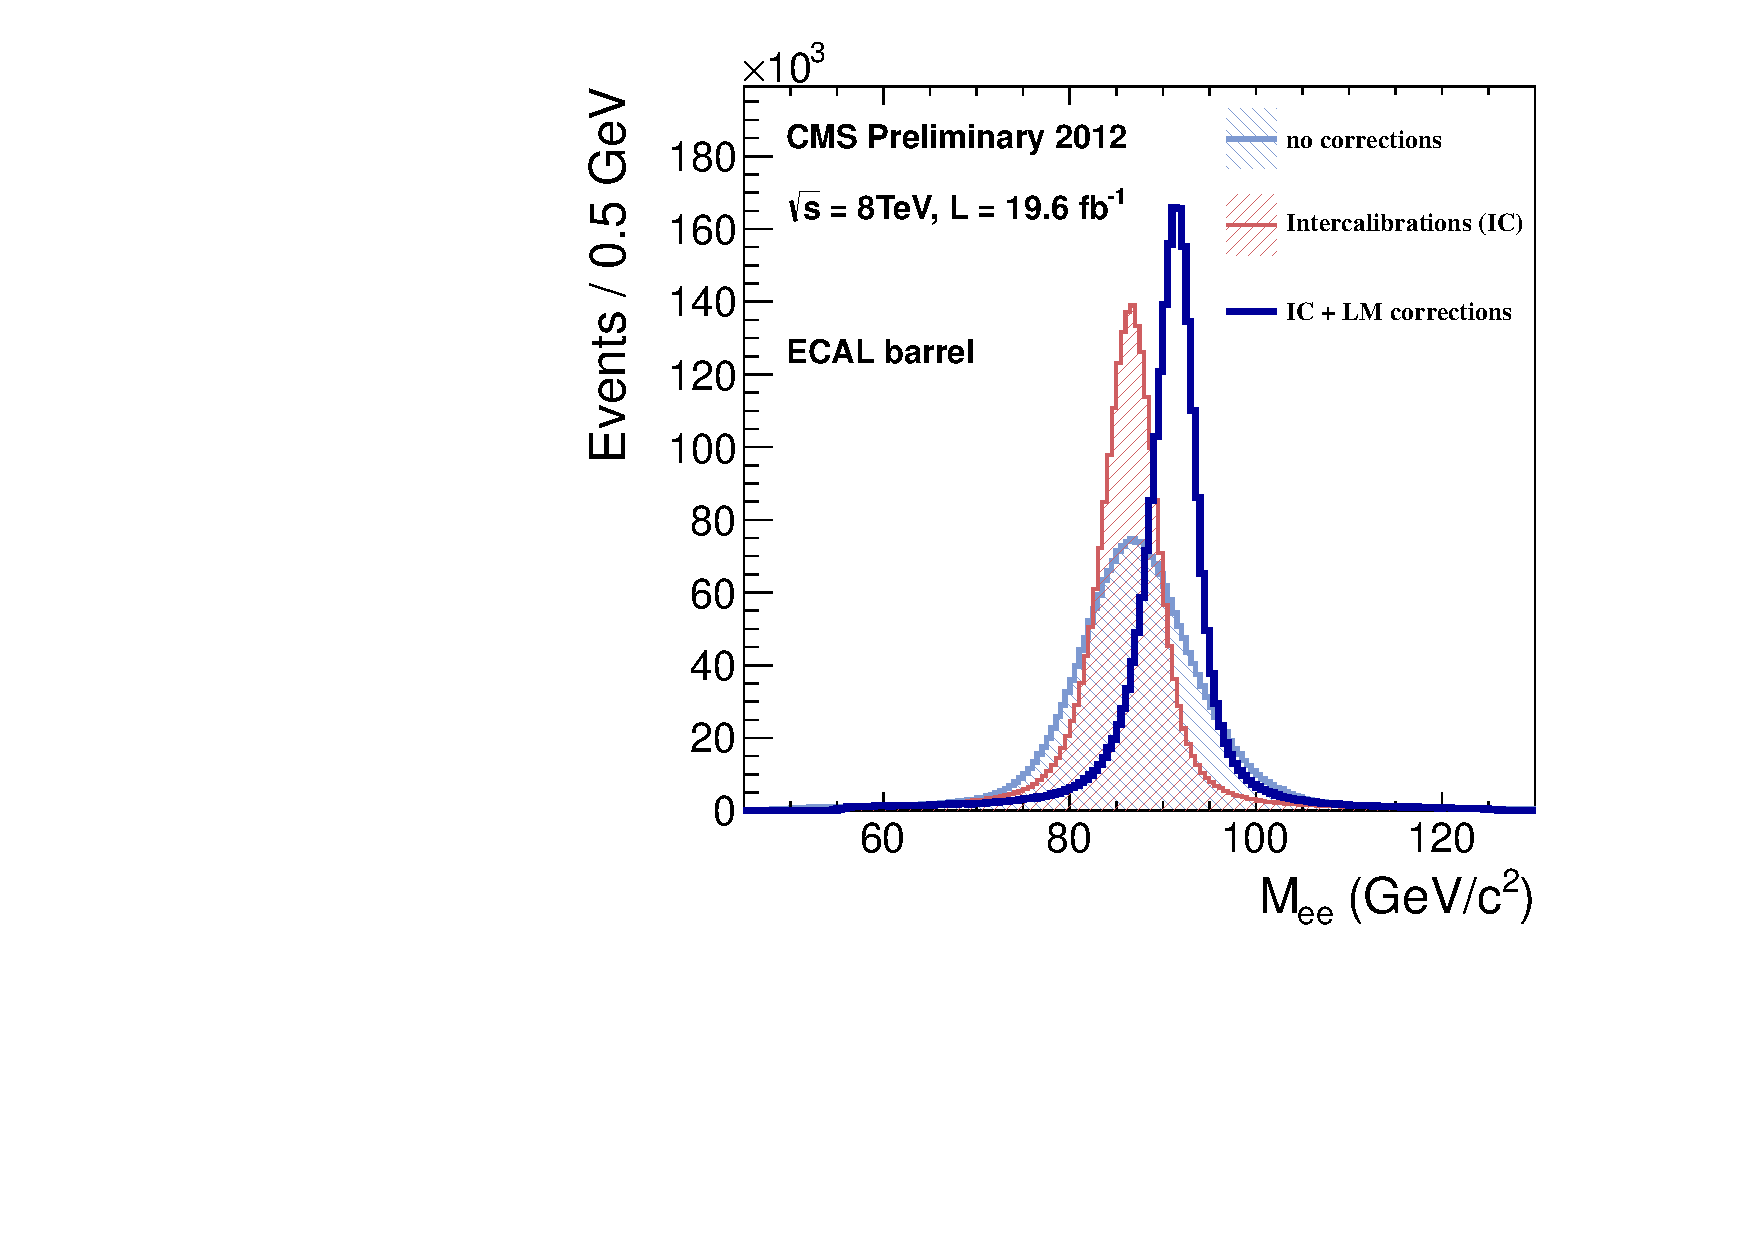
\includegraphics[height=0.35\textwidth, width=0.50\textwidth]{THESISPLOTS/propaganda_noIC_noLaser-regrCorr_ele-EB.pdf} 
%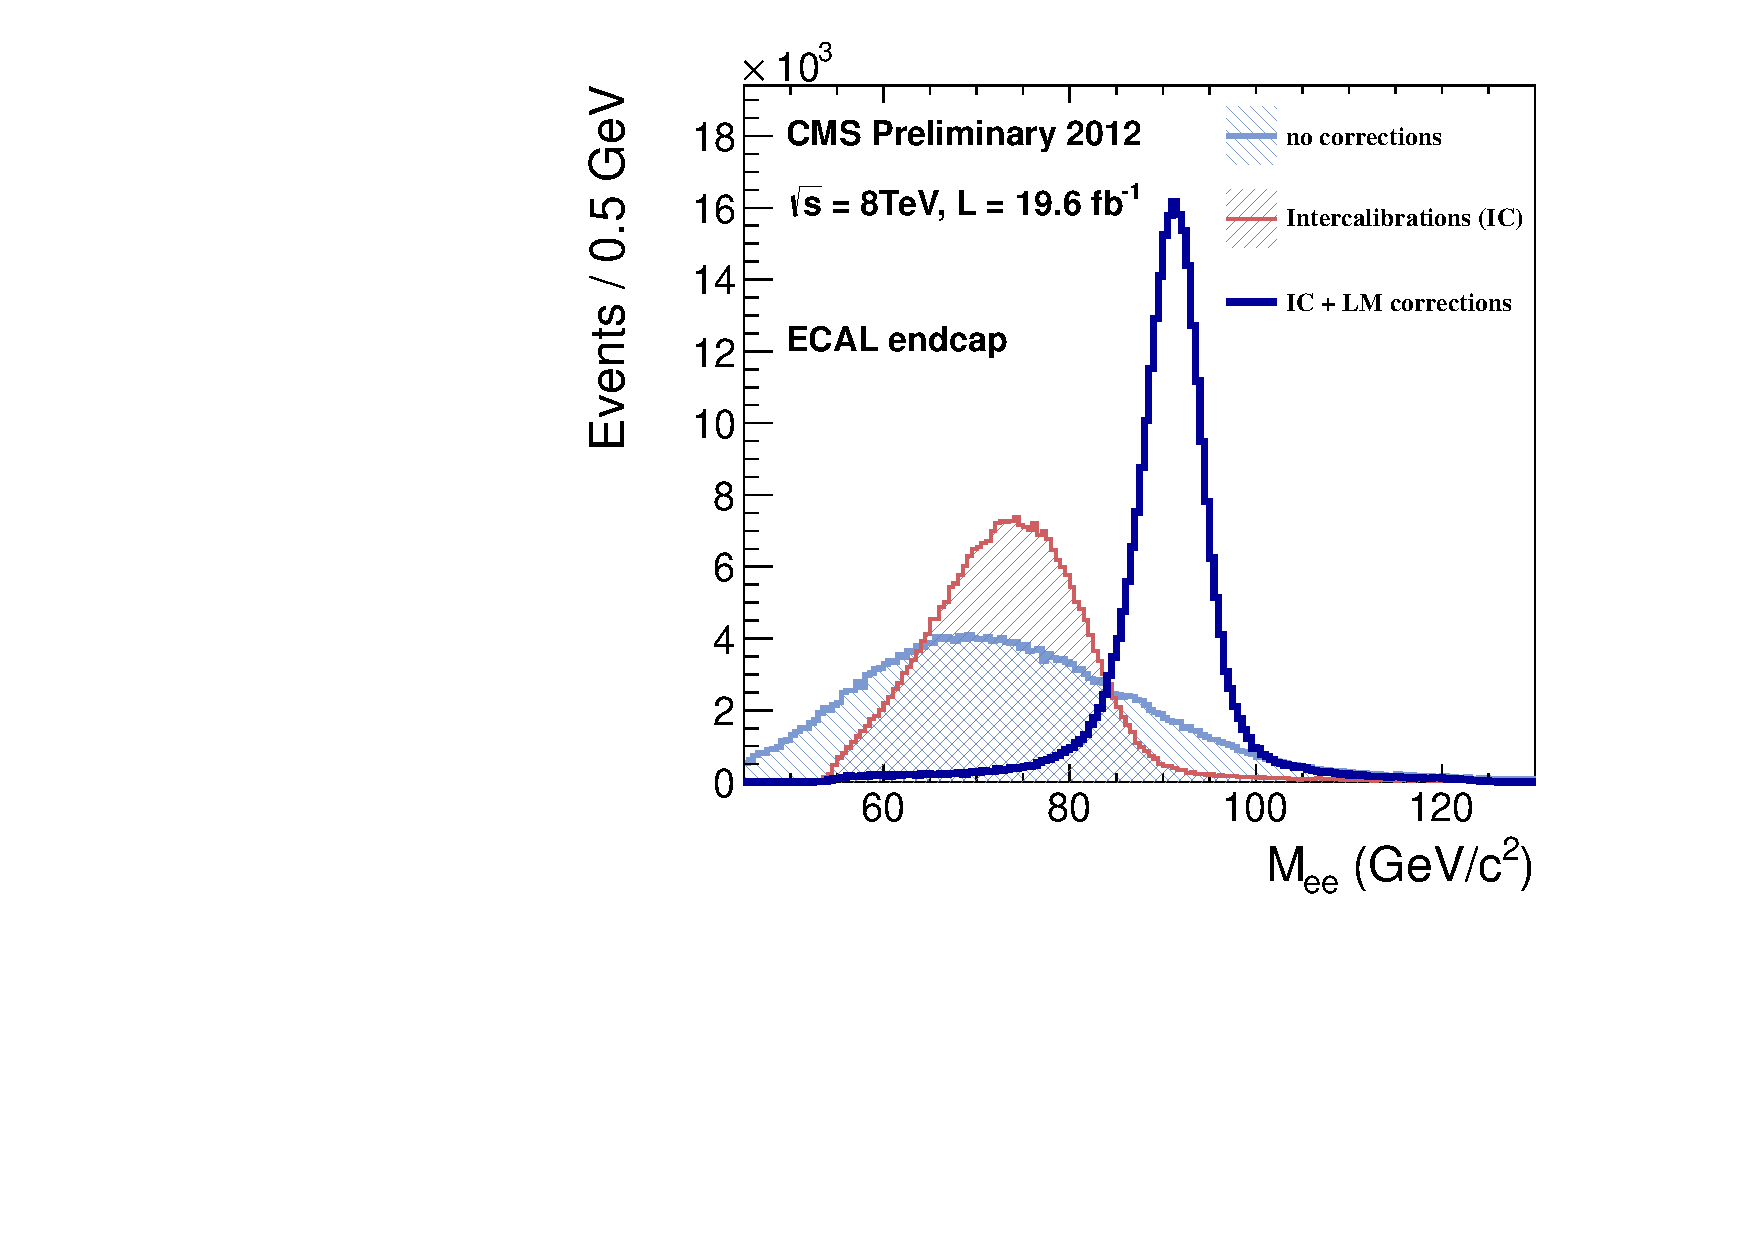
\includegraphics[height=0.35\textwidth, width=0.50\textwidth]{THESISPLOTS/propaganda_noIC_noLaser-regrCorr_ele-EE.pdf} }
%\captionof{figure}{\PZ mass distribution from $\PZ\rightarrow e^{+}e^{-}$  decay showing improvement in the measurement of the $\PZ$ mass after performing energy adjustments to account for intrinsic spread in crystal, photo-detector response and time-dependent corrections to compensate for channel response loss for EB~(right) and EE~(left)}
%\label{fig:EnergyCorr}
%\end{center}
%\end{minipage}

%\vspace{5mm}
%\begin{minipage}{0.94\textwidth}
%\begin{center}
%\mbox{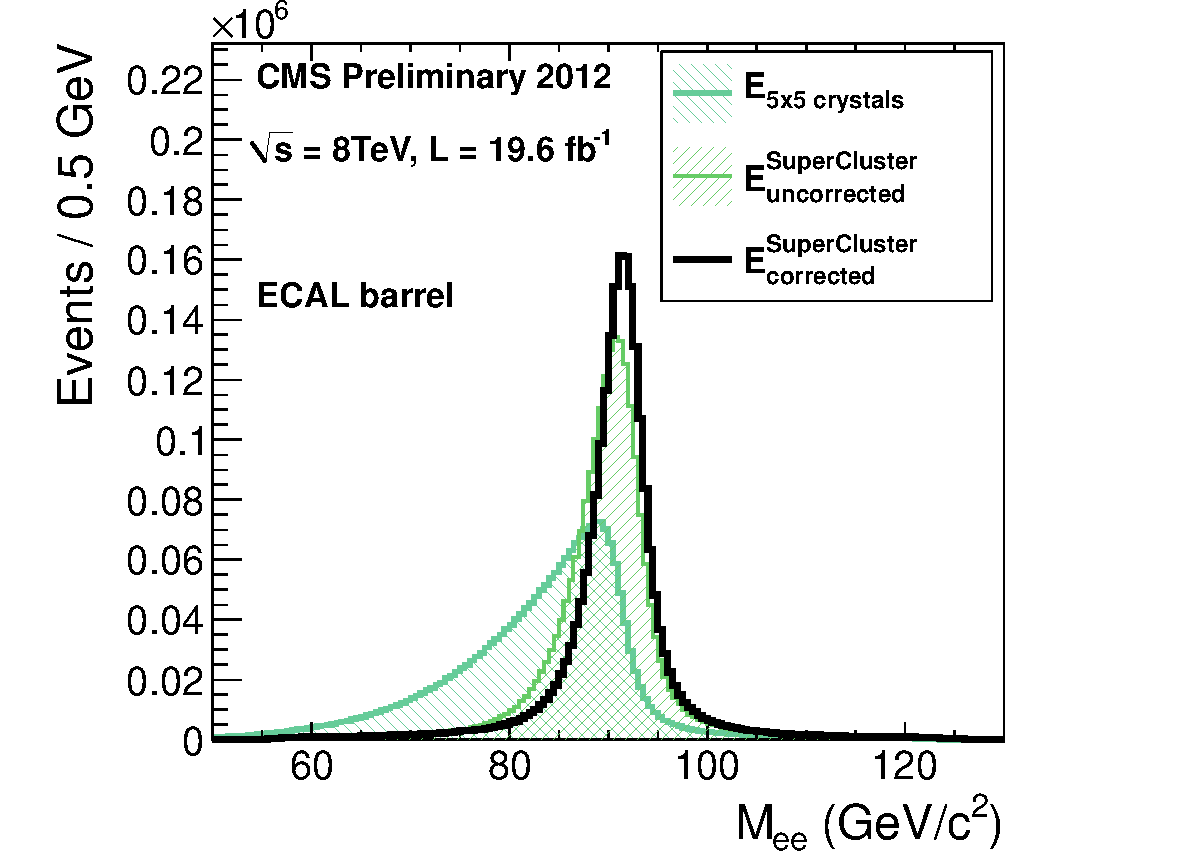
\includegraphics[height=0.35\textwidth, width=0.50\textwidth]{THESISPLOTS/E_corr-EB.pdf}
%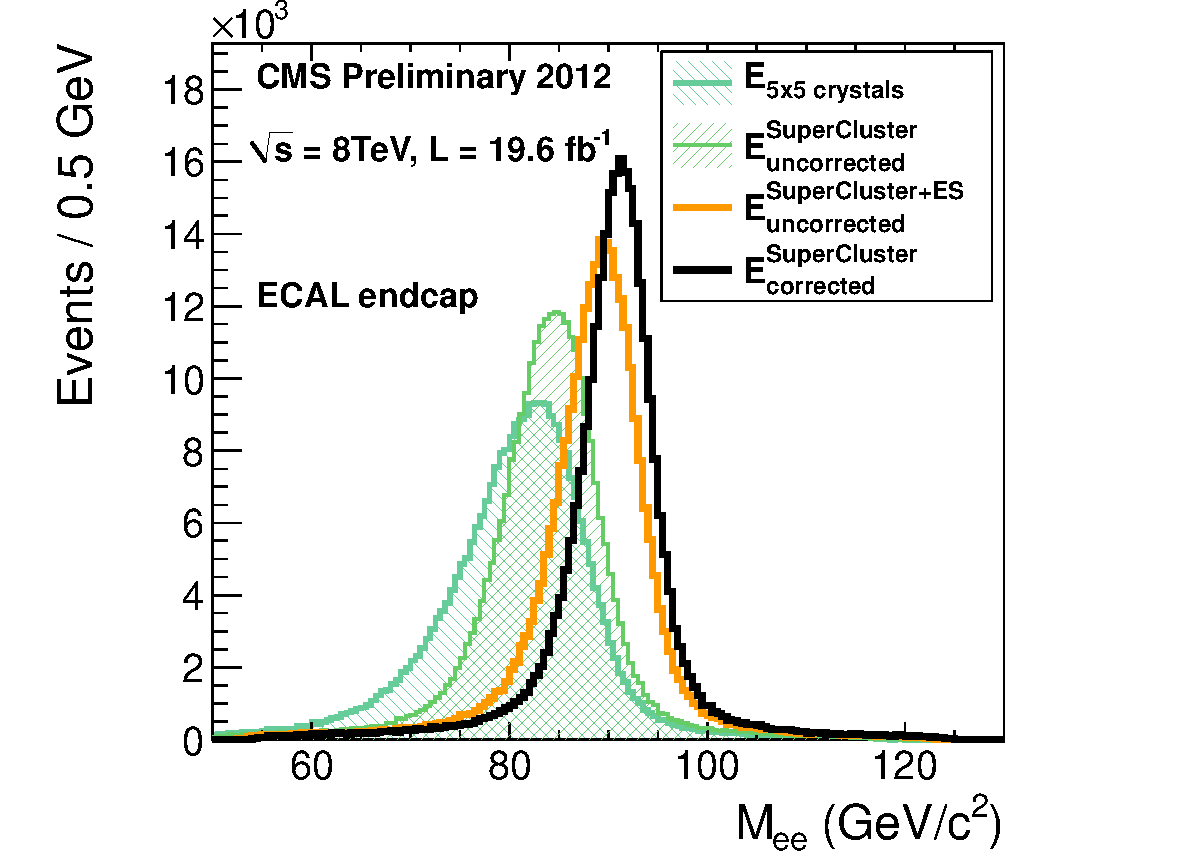
\includegraphics[height=0.35\textwidth, width=0.50\textwidth]{THESISPLOTS/E_corr-EE.pdf} }
%\captionof{figure}{\PZ mass reconstructed using electron superclusters shows improvement in \PZ mass measurement after applying energy adjustment at superclusters for EB~(right) and EE~(left).}
%\label{fig:SCEnergyCorr}
%\end{center}
%\end{minipage}

%\vspace{5mm} 
%%%%%%%%%%%%%%%%%%%%%%%%%%%%%%%%%%%%%%%%%%%%%%%%%%%%%%%%%%%%%%%%%%%%%%%%%%%%%%%%%%%%%%%%%%%%%% 
%Why even talk about these electron ID variables when you aready described them in your event selection for photons? 
%%%%%%%%%%%%%%%%%%%%%%%%%%%%%%%%%%%%%%%%%%%%%%%%%%%%%%%%%%%%%%%%%%%%%%%%%%%%%%%%%
%%\par 
%%Electrons and photon identification uses many selections variables which can be described as follows:
%%\par 
%% In Table \ref{tab:EgammaID}, we present a summary of variables constructed using information of the 
%%spread of the electromagnetic shower in $\eta$ and $\phi$, the ratio of the energy deposited in  HCAL to ECAL, the track $\PT$ and  ECAL $\ET$, isolation in ECAL, HCAL and tracker, the ratio of the energy sums over $3\times3$ and $5\times5$ matrices centered on the highest energy  crystal of the seed cluster; $R_{9} = E_{3\times3}/E_{5\times 5}$ or $R_{9} = \sum E_{9}/\sum E_{Supercluster}$ and impact parameter,  $d0$, which is the minimum separation of the electron track computed with respect to the  reconstruction vertex and track transverse momentum, $p_{T}$. Photon and electron selection using these variables, applied during electron and photon identification, have been shown to produce very good quality electron and photon candidates with efficiency above 70\%.

%With these electron or photon candidates, further selections using variables constructed from 
%information on the 
%to further identify photons and electrons.  
%Additional pre-electron candidates based on cut elections such as minimum transverse energy, $E_{T} > 4$~ GeV, $\eta$ and $\phi$ geometrical matching; $\Delta Eta < 0.02$, $\Delta \phi < 0.1$  and a cut on Ratio of hadronic to electromagnetic energy cluster: $H/E < 0.2$ is enough to suit physics analysis, however, additional elections and identification criteria are added depending on the purpose of the particular analysis to fully defined an electron or photon.
%These identifications and isolation criteria can also be categorised in terms of flavours as being very loose~(VL), loose~(L), medium ~(M) and tight~(T).
%The typical variables used for electron and photon identification are defined as follows:
%\begin{itemize}
%\item Ratio of energy of HCAL behind super cluster to super cluster energy: $H/E$
%\item Energy momentum matching variables between energy of the super cluster  or of the super cluster seed and electron track  measured momentum  at the vertex or  at the calorimeter: $E/p_{in}$, $E_{seed}/p_{in}$, $E_{seed}/p_{out}$
%\item Geometrical matching between the electron track parameters at the vertex  extrapolated  to the super cluster  and the measured  super cluster position: $\Delta \eta_{in}$, $\Delta \phi_{in}$.
%\item Calorimeter shower shape  variables: the width of  the ECAL cluster  along the $\eta$  direction  computed  for all  the crystals  in the $5\times 5$  block of crystals centered  on the highest energy crystal  of the seed cluster ,$\sigma_{i\eta,i\eta}$  This $R_{9}$ variable makes a good separation between  unconverted photons~(energy not spread in tracker) and converted photons~(energy spread by B-field before reaching ECAL).
%\item Bremsstrahlung fraction: (track momentum at vertex -  track momentum at  ECAL)/ track momentum at vertex.
%\item 1/E(Super cluster) - 1/p(track at vertex)
%\end{itemize}
%As an improvement on the photon and identification,  also serves as additional isolated photon and electron selections. Separating true photons from collision arriving at ECAL from converted photons,  additional selections on variables like , are used.
%\begin{itemize}
%\item  Calorimeter shower shape:$R_{9}$
%\item Impact parameter: $d0$, minimum separation of the electron track computed with respect to the  reconstruction vertex.
%\item Missing Hits: Number of cross layers  without a compatible hits in the back-propagation of the track to the beam-line.
%\end{itemize}
% Isolation variables in addition to the identification variables are used to improve on the performance of identification. Below are the following isolation variables as defined and used by the CMS:
%\paragraph*{ Electron Photon Isolation} 
% \begin{itemize}
% \item Tracker Isolation: sum of $p_{T}$ of tracks  with $p_{T} > 0.7~GeV/c$ and maximum distance to the vertex  of 0.2~cm in  a cone of 0.3 with an inner veto cone of 0.04.
% \item ECAL Isolation: sum of energy  of ECAL RecHits with a Jurassic footprint removal ~(Jurassic width of about 1.5 crystals) in a cone  of 0.4  with veto cone of 3 crystals. A RecHit noise cut of 0.08~GeV in energy~(E) in barrel and 0.1~GeV in transverse energy~($E_{T}$) in the endcap is applied.
 %\item HCAL Isolation: sum of HCAL Calorimeter Towers in a 0.4 cone with a 0.15 veto cone.
 %\end{itemize}
%In general the major difference between an electron and a photon as identified by the CMS detector is that electrons which have no pixel strip hits are automatically  classified as photon candidates and further isolation and shower shape variables are used to arrive at the ultimate photon as required by a given analysis.
%The full table using simple selection cuts on these variables used for standard electron and photon identification and isolation which is also used in our analysis is shown in table \ref{tab:EgammaID}.
 % is a summary of the simple cut-based selection criteria on variables and their selection thresholds used for identifying isolated electrons and photons in CMS which has also be used in our search analysis for event selection.
 
%%\vspace{5mm}
%%\begin{minipage}{0.94\textwidth}
%%\begin{center}
 %\setlength{\abovecaptionskip}{0pt}
  %\setlength{\belowcaptionskip}{10pt}
 % \topcaption{GMSB,GGM Phenomenology and Relevant final states}
%%\begin{tabular}{l|l|p{3.2cm}} %p{3.9cm}}
%%  \multicolumn{3}{c}{\bfseries{Simple Cut Based Electron Photon Identification}} \\
%%  \toprule
%%  \hline
%%  \bfseries{ID Variable} & \bfseries{Electron} & \bfseries{Photon} \\
%%   \hline
%%  $H/E$ & 0.05(EB), 0.10(EE)  & 0.05 \\
%%  \hline
%%  $|\Delta \eta_{in}|$ & 0.005(EB), 0.007(EE)  & 0.015(EB)  \\
%%  \hline
%%   $|\Delta \phi_{in}|$ & 0.09(EB), 0.09(EE)  & N/A \\ \hline
%%   $\sigma_{i\eta i\eta}$ & 0.01(EB), 0.03(EE) & 0.011(EB), 0.03(EE)  \\
%%   \hline
%%   Pixel Veto & No & Yes \\
%%   \hline
%%   $|d0|(vertex)$ & 0.02(EB), 0.02(EE) &  Veto \\
%%   \hline
%%    $|dZ|(vertex)$ & 0.1(EB), 0.1(EE) & 0.02~(cm)(Veto) \\
%%    \hline
%%     $|1/E - 1/p|$ & 0.05(EB), 0.05(EE) & N/A \\
%%     \hline
%%     PF isolation / $p_{T}$ (cone dR=0.3) & 0.15(EB),0.10(EE) &  N/A \\
%%     \hline
%%     ECAL Isolation & same  & $4.2 + 0.006*E^{\gamma}_{T} + 0.183*\rho$(EB) \\
%%     \hline
%%     HCAL Isolation & same & $2.2 + 0.0025*E^{\gamma}_{T} + 0.062*\rho$ \\
%%     \hline
%%     TRACK Isolation & same  & $2.0 + 0.001*E^{\gamma}_{T} + 0.0167*\rho$ \\
%%     \hline
%%     Rho corrected PF photon isolation & N/A & $1.3 + 0.005*p^{\gamma}_{T}$(EB) \\      
%%   \hline
%%   \bottomrule
%%  \end{tabular}
%%   \captionof{table}{ Simple cut-based selection criteria for electron and photon identification.}
%% \label{tab:EgammaID} % for use in \ref{table1} if you want to refer to the table number
%% \end{center}
%\end{table}
%%\end{minipage}

\section{Muon Reconstruction}
%%%%%%%%%%%%%%%%%%%%%%%%%%%%%%%%%%%%%%%%%%%%%%%%%%%%%%%%%%%%%%%%%%%
Muon tracks are reconstructed using the all-silicon inner tracker~(tracker tracks) and the muon system~(standalone tracks). The standalone tracks are reconstructed using reconstructed positions~(hits) in the muon system consisting of the Drift Tubes~(DT) in the barrel~($|\eta| < 0.9 $), Cathode Strip Chambers~(CSC) in the endcaps~($1.2 <|\eta| < 2.4$) and Resistive Plate Chambers~(RPC) in the overlap region~($0.9 <|\eta| < 1.2 $).
There are two independent muon reconstruction approaches: \textit{Global muon reconstruction~(Outside-in)} and \textit{Tracker muon reconstruction~(Inside-out)}.
For Global muon reconstruction, each standalone-muon track is matched to a tracker track by comparing the parameters of the two tracks propagated to a common surface. The global muon track is fitted combining hits from the tracker track and standalone-muon track using the Kalman-filter algorithm. 
For the tracker muon reconstruction, all tracks with $\pt > 0.5$\GeVc and total momentum $p > 2.5$\GeVc
are considered  as possible muon candidates and are extrapolated to the muon system taking into consideration the magnetic fields, the average expected energy loss in the calorimeters and multiple Coulomb scattering in the detector material to locally reconstruct segments in the muon system.
A combination of different muon algorithms depending on the muon \pt, provides a robust and efficient muon identification.
\newline
Using the beam spot as constraint for the muon's vertex, we can distinguish between muons produced from $pp$ collisions from \textit{cosmic muons} and \textit{beam halo muons}~(muons produced from the interaction of the proton beam with the gas in the beam pipe). Figure \ref{fig:Muons} show an illustration of the trajectories of different muon sources interacting with the CMS detector.
 
\vspace{5mm}
\begin{minipage}{0.94\textwidth}
\begin{center}
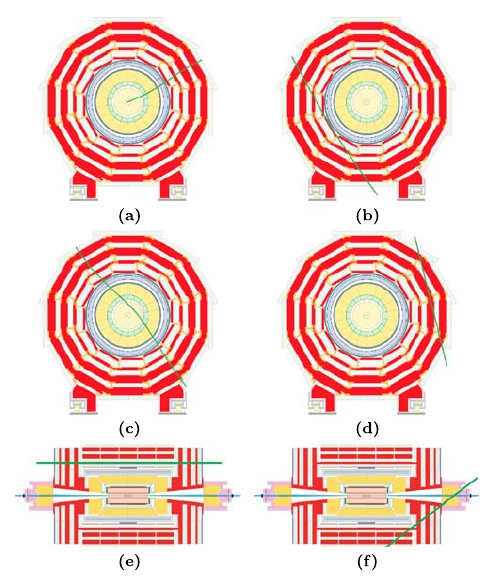
\includegraphics[height=0.40\textwidth, width=0.80\textwidth]{THESISPLOTS/Cosmic_Halo_Muons.png}
\captionof{figure}{Illustration of muons from proton-proton collision, cosmic rays and beam halo. (a) Muons from collision propagating from the center and moving outwards, (b) Cosmic muons traveling through the detector leaving signals in opposite hemispheres of the muon system, (c) Cosmic muons leaving signals in the tracker and opposite hemispheres, (d) cosmic muons entering and leaving the detector without passing through the muon detector layers, (e) beam halo muons penetrating the detector and leaving signals in the endcaps and (f) Cosmic muons entering the detector through the endcap~(EE) and leaving through the barrel~(EB). This can happen in the reverse way; EB to EE.}
\label{fig:Muons}
\end{center}
\end{minipage}
%A new stand-alone and global muon reconstruction software with the assumption that muons originate from outside the CMS detector and according to the properties of cosmic and halo muons has been optimised to reconstruct and identify both cosmic and halo muons which are used studies involving calibration and aligning the muon detectors
%PF algorithm takes into consideration  information from every sub-detectors like the tracker, ECAL, HCAL and muon section before identifying a particular physics objects.
\section{Particle Flow Algorithm}
The \textit{Particle Flow}~(PF) algorithm is an algorithm for reconstructing particles using detector information from the tracker, ECAL, HCAL and muon chambers of the CMS detector \cite{PFALGO,PF}.
It uses a combination of different algorithms comprising of calorimeter clustering, tracking and extrapolation to calorimeters, muon identification, electron pre-identification and linking local reconstructed elements, for reconstructing a list of particles which include photons, charge hadrons, neutral hadrons, muons and electrons. The same list of particles is subsequently used to reconstruct composite "particles" like jets, \MET and taus. The versatility of the PF algorithm is the reason why it was introduced for reconstructing Jets and missing transverse energy~(\MET), where complete information of the event content from every subdetector is needed for best performance. The PF algorithm uses tracks, electron energy seeds, 4-momentum, super cluster energy calibration, bremsstrahlung tracks for electron and photon reconstruction making it extremely efficient at minimizing electron and photon misidentification.
For \MET reconstruction where full reconstruction of all the particles belonging to an event is necessary, the PF algorithm is very reliable. 
\section{Jet Reconstruction}
%%%%%%%%%%%%%%%%%%%%%%%%%%%%%%%%%%%%%%%%%%%%%%%%%%%%%%%%%%%%%%%%%%%%%%%
A jet is a spray of particles arising from the hadronization of colored particles. 
Because jets are made of many particles like hadrons and photons from \Ppizero decay, they are best reconstructed using the particle flow algorithm.
Jets reconstructed using the PF algorithm are called \textit{PF-Jets}. 
\newline
Using calorimeter towers as input, jets can be reconstructed using the Anti-$k_{T}$ clustering algorithm which combines four vectors according to their relative transverse momentum~(\pt) within a standard cone size of $\Delta R = 0.5$ in the $(\eta, \phi)$ plane, where, $\Delta R = \sqrt{ \Delta\eta^{2} + \Delta\phi^{2} }$.
\newline 
The quality of a reconstructed jet depends on a set of selection variables collectively referred to as the \textit{JetID}. The JetID consist of variables which selects on jets candidate base on the composition of the jets. The jet composition can be described using the following quantities: electromagnetic energy fraction~(EMF), the charge  hadron fraction~(CHF), the neutral hadron fraction~(NHF), the charge electromagnetic fraction~(CEF),  neutral electromagnetic fraction~(NEF) the number of calorimeter cells containing more than 90\% of jet energy~($N^{90}_{jet}$), the fraction of jet energy in the hottest  Hybrid photodetector~(HPD) unit in HCAL readout within a jet~($f_{HPD}$) and the $\eta$ region of the jet. The selection threshold and combination of jetID variables used  will depend on a specific analysis and the type of jets involved.
In general, jet candidates are required to have an electromagnetic energy fraction~(EMF) more than 10\% \ie $EMF > 0.01$,  must be within the ECAL fiducial region of $|\eta| < 2.6$, the number of calorimeter cells containing more than 90\% of jet energy~($N^{90}_{jet}$) must be $ > 1$, the fraction of jet energy in the hottest  Hybrid photodetector~(HPD) unit  in HCAL readout within a jet~($f_{HPD}$) must be $ > 0.98$, the charge  hadron fraction~($CHF$)$ >0.0$ if within $|\eta| < 2.4$, the neutral hadron fraction~($NHF$)$ < 1.0$ , the charge electromagnetic fraction~($CEF$) $ < 1.0$, and neutral electromagnetic fraction~($NEF$) $< 1.0 $.
These jetID selection requirements have been shown to remove mis-reconstructed jets arising from spurious energy deposition in subdetectors with good efficiency \cite{JET}.
\newline
The jet energy is often mis-measured due to non-linear responses in the calorimeters as the hadronic shower develops, cracks in the detector and additional energy from events with PU. The jet energy is corrected for contributions from the above sources through \textit{Jet Energy Corrections}~(JEC) measurements \cite{JEC}. Applying these corrections during reconstruction guarantee a reliable measurement of the jet energy , however, JEC is one of the sources of uncertainties in most analysis which involve jets. 
%CMS reconstructs four types of jets which each combine individual contributions from sub-detectors  to form inputs to a jet clustering algorithm. The four types of jets include Calorimeter jets, Jet-Plus-Track~(JPT) jets, Particle-Flow~(PF) jets and track jets. 
%Calorimeter jets are reconstructed using energy deposits in the combine ECAL and HCAL calorimeter cells called calorimeter towers. A calorimeter tower is a single or group of HCAL cells with their geometrically corresponding ECAL crystals. In order to suppress both noise and and contributions from event pile-up~(additional proton collisions within the same bunch crossing), thresholds are applied to both the individual cells when building the calorimeter towers as well as a transverse energy~($E_{T}$) cut on the calorimeter tower energy. Typical $E^{towers}_{T} > 0.3 - 0.7$~ GeV is often used.


%PFJ are reconstructed using the PF algorithm. The PF algorithm uses as input a list of reconstructed particles which include charge hadrons from tracks  in central tracker, photons and neutral  hadrons reconstructed from energy clusters in the HCAL and ECAL, neutral particles as clusters separated from extrapolated position of tracks in calorimeters  and electrons from tracks matched to clusters in the calorimeters.
%The PF algorithm exploits the high granularity in ECAL to precisely measure charge hadrons and photons inside jets, which makes up a larger portion of the jet energy.

%This JEC to determine the jet absolute response is a source of systematic uncertainties in a given physics analysis.
\section{Missing Transverse Energy Reconstruction}
%%%%%%%%%%%%%%%%%%%%%%%%%%%%%%%%%%%%%%%%%%%%%%%%%%%%%%%%%%%%%%%%%%%%%
Missing Transverse Energy is defined as the negative vector sum of the transverse energy deposits of all the particle candidates in an event, including the JEC. Its magnitude, \MET is given as
\begin{equation}\label{met}
 \MET =| - \sum_{n}(E_{n}\sin\theta_{n}\cos\theta_{n} \hat{\mathbf{i}}  + E_{n}\sin\theta_{n}\sin\theta_{n} \hat{\mathbf{j}} ) | = |\ETslash^{x}\hspace{.08em}\hat{\mathbf{i}} + \ETslash^{y}\hspace{.08em}\hat{\mathbf{j}} |
\end{equation}
Where, $n$ is the sum over all calorimeter energy deposits including  energy deposits in towers, reconstructed energies~(hits) or generator level particle energies. \MET is use to infer the presence of a particle which escaped the CMS detector like neutrinos~(\Pneutrino), neutralinos~(\PSneutralinoOne) and gravitino~($\tilde{G}$).
\par 
In order to measure \MET accurately, a particle detector should be nearly hemetic \ie have a $4\pi$ solid angle coverage, to allow for complete measurement of the transverse momentum of all the particles belonging to an event. The hadronic forward~(HF) subdetector  of the CMS detector, with little space allowing for the passage of the proton beams, provide this near $4\pi$ solid angle.
\newline
Measuring \MET  is always challenging and is a source of uncertainty in most analysis which involve \MET as machine induced background processes, mis-measured energy of and from mis-reconstructed particles and anomalous signals like spike can contribute to the measurement of \MET. By minimizing the contributions from these processes we can measure \MET better \cite{MET2,MET}.
\newline
The use of \MET in event selection is common in most analysis which involves the search for new phenomena which is a common prediction in models Beyond Standard Model~(BSM) like \textit{supersymmetry}. The presence of large \MET in an event indicates the presence of a new particle not described by standard model interactions which usually have small \MET as in the case of the neutrino in the \PW boson decay, $\PW \rightarrow \Pe + \APnu$.

%%%%%%%%%%%%%%\
%The definition of \MET and its reconstruction is based on the conservation of transverse momentum transverse. It is interpreted as the imbalance in transverse momentum to ensure conservation of total transverse momentum in an event and the transverse momentum imbalance arise from the momentum carried away by undetected particle traveling in the transverse plane.
%Since according to conservation of momentum, the total transverse momentum before and after collision should be the same, by measuring the \pt of every detectable particle belonging to an event after proton-proton collision, the imbalance in \pt required to ensure the conservation of transverse momentum in the event, is ascribed to the momentum carried away by undetected particle(s). This idea is used to infer the presence of neutrinos \PW boson decay to an electron and an anti-electron neutrino; $\PW \rightarrow \Pe + \APnu$, where the missing transverse momentum is used to infer the presence of the undetectable neutrino.
%%%%
%Anomlous signals are signals read from the electronics called \textit{spikes} with abnormally large energy deposits in the avalanche photodiodes without any scintilation in the \pb crystals.

%%%%%%%%%%%%%%%%%%%%%%%%%%%%%%%%%%%%%%%%%%%%%%%%%%%%%%%%%%%%%%%%%%%%%%
%%%%%%%%%%%%%%%%%%%%%%%%%%%%%%%%%%%%%%%%%%%%%%%%%%%%%%%%%%%%%%%%%%%%%%%
\section{Anomalous Signals}\label{spikes}
Sometimes anomalously large signals called "\textit{spikes}" are produced when neutrons or charged hadrons like protons strike directly, ionizing the silicon of the photodiode  producing an electronic signal even in the absence of any crystal scintillation.
% These kind of events produced large isolated energy deposits thus are referred to as "punch through" events or "spikes".
\newline
Because spike signals are not produced through the crystal scintillation process, which takes about 10~ns, their measured arrival time is early and negative. Energy deposits from spikes range from a few \GeV to the saturation energy of ECAL which is about $1.7$\TeV. Since they are not due to showering particles, most often only one isolated crystal sees such energy.  Spikes may occasionally have positive time, appearing late or delayed in their arrival time at ECAL, and populating the tails of the photon's rechit time distribution. The late arrival time may be due to the slow propagation~(takes an indirect route) of neutrons through the CMS detector. 
\par 
Numerous test beam, collision data and simulation studies \cite{spike,spike2}, have been carried out towards understanding the properties of events with spikes and how they can be tagged and removed. 
These studies reveal that most spikes can be identified using a topological energy sharing variable called "\textit{Swiss-Cross}"~(SX) constructed as $1 - \frac{E_{4}}{E_{1}}$. $E_{1}$ is the energy deposit of the central~(highest energy) crystal and $E_{4}$ is the sum total of the energy of the neighboring four crystals in the $(\eta , \phi)$ plane. A selection cut SX $ > 0.95$ rejects more than 99\% of isolated spikes with transverse energy greater than 10\GeV with very little impact on the efficiency of selecting electromagnetic~(EM) showers.
Other topological energy sharing variables like $ 1 - \frac{E_{6}}{E_{2}}$ and $ 1 - \frac{E_{9}}{E_{2}} $, where $E_{2}$ is the sum of the energy of two  crystals sharing the energy deposited from simultaneous spikes and $E_{6}$($E_{9}$) is the sum of the neighboring 6(pairs-of)(9) crystals in the $(\eta , \phi)$ plane. The $1 - \frac{E_{6}}{E_{2}} $ variable is used to identify isolated spikes whose energy deposit spread in two adjacent crystals while the  $ 1 - \frac{E_{2}}{E_{9}} $ is used to identify  non-isolated spikes \ie spikes which are found embedded in a supercluster.
\newline
It has also been shown that applying selection cuts on the rechit time of $ \pm 3$~ns leads to more than 90\% efficiency for rejecting spikes. However, in this thesis, we do not require such selection cuts on the rechit time as these rechits include rechits of possible delayed electromagnetic particles produced during $pp$ collisions with arrival time beyond 3~ns.

%%%%%%%%%%%%%%%%%%%%%%%%%%%%%%%%%%%%%%%%%%%%%%%%%%%%%%%%%%%%%%%%%%%%%%%%%%%%%%%%%%%%%%%%%%%%%%%%%%%%%%%
\label{Reconstruction_and Particle_ID_chapter}
%%%%%%%%%%%%%%%%%%%%%%%%%%%%%%%%%%%%%%%%%%%%%%%%%%%%%%%%%%%%%%%%%%%%%%%%%%%%%%%%%%%%%%%%%%%%%%%%%%%%%%%

%As a result, most of the results presented in this thesis are taken directly from \cite{spike} or redone for 2012 dataset which this analysis is based upon. It has been observed through studies using minimum bias data set( highly populated with neutrons and  charged hadrons) at different center of mass energy, that the number of spikes increases with the proton collision rate as well as the charged tracks per event i.e there is a strong linear correlation between spike rate and the center of mass energy of pp collision. The reason for this is because more neutrons and charged hadrons with enough energy are produced which "punch through" the APD and produce hikes in the rechit energy profile as read from the APDs. It is understandable that spike production is most common in the barrel compared to the endcap. Thus with increases rate of proton collision and  $\sqrt{S} = 8$~\TeV, it is imperative to have robust variables which can identify and reject spikes in the barrel in this analysis.  
%The  above studies show that variables defined using timing and EM energy deposits are reliable. Other variables using the timing pulse shape and EM shower profile can be use in addition to identify and rejects spikes with  efficiency of 90 to 95\%.
%\newline
%Rejection of spikes is done at online( CMS Level-1 trigger level) as well as offline and analysis level.
%\newline
%At online, the strip Fine-Grained Veto Bit(sFGVB) is set to 0 or 1 use to flagging an object as either a spike or a good event respectively. A detail of this can be found in \cite{spike2}. For example if the sFGVB is set to 0 and the  trigger tower( $5 \times 5$ crystals) transverse energy is below 12~\GeV, the energy deposition is considered spike-liked and the corresponding tower will not contribute  to CMS triggering of that event. The sFGVB was implemented in 2011 data taking process and was measured to reject over 95\% of spikes with transverse energy greater than 8~\GeV(12~\GeV) in 2011(2012).
%The figure {\textbf{Figure of sFGVB}} shows the difference between an good EM-cluster and a spike-like cluster at sFGVB level.
%\newline
%At Offline, variables making using of the single(at times double) channel(crystal) energy deposit and early arrival time of spikes are defined.
%In figure {\textbf{Figure of Swiss X and Rechit Time}}, we show the difference between spikes and normal events energy clusters explaining the variables used to identify spikes in the offline.

%The figure{\textbf{Figure of Spike energy topology and Distribution of SwissX}} shows the construction of the swiss-cross variable as well its distribution in data and simulation events. The peak at 1.0 in data of the distribution is due to the presence of spikes. 
%Other topological energy deposit variables such as $ 1 - \frac{E_{2}}{E_{6}}$ and $ 1 - \frac{E_{2}}{E_{9}} $ where $E_{2}$ is the sum of the energy of two  crystals sharing the energy deposited and $E_{6}$($E_{9}$) is the sum of the neighbouring 6(pairs-of)(9) crystals in the $\eta - \phi$ plane.
%The $ 1 - \frac{E_{2}}{E_{6}} $ variable is used for the identification of  isolated spikes whose energy deposit spread in two adjacent crystals while the  $ 1 - \frac{E_{2}}{E_{9}} $ is used to identify  non-isolated spikes or spikes which are found embedded in a normal Ecal supercluster.

%The figure {\textbf{Put figure of di-spike and non-Isolated spike construction and distribution}}  
%A cut on $ 1 - \frac{E_{2}}{E_{6}} $ ( $ 1 - \frac{E_{2}}{E_{9}} $)  greater than 0.95 ( 0.98 for tight) gives an efficiency close to 95\% for events with transverse energy greater than 10~\GeV for rejecting spikes with very little effect on normal EM shower reconstruction.
%\newline
%Another very important variable used for rejecting spikes with greater efficiency is rechit ECAL timing. Spikes and EM energy deposits show very distinct signal pulse shapes. Since spikes do not  in the \pb , when the pulse shape is fitted to extract the timing of a signal, the spikes appear "early" due to faster rise time of the spike pulse.
%The figure {\textbf{Fig of spike pulse shape and rechit time distribution for data and simulation}} shows the comparison between the pulse shape for a spike candidate pulse and and true \pb scintillated event. The adjacent plots shows the distribution of the rechit time for simulation( where  there are no anomalous signals) and collision data where anomalous signals have a significant contribution to out-of-time signals.% timing distribution.

%\newline
%However, it is worth nothing that, these anomalous signals if not rejected will lead to a biasing in the reconstruction of other physics variables such as missing transverse energy(~\MET) as well as being miss-identified as a possible signal for delayed photons.
%Infact the spike rate per bunch crossing as observed in \cite{spike2} was approximately $ 1 \times 10^{-3}$ in collisions bunch crossings while in non-collision bunch crossing is of the order of $2 \times 10^{-6}$ in non-collision bunch crossings. This spike rate from non-collision rate is obtained from cosmic muon data recorded during June-August 2009 while the spike rate for collision is obtained from Minimum biased( Soft proton-proton) collision events data.
%Thus, in this thesis, we have restricted ourselves to using only the energy topological variables discussed in previous paragraphs to identify and reject anomalous signals.
%%%%%%%%%%%%%%%%%%%%%%%%%%%%%%%%%%%%%%%%%%%%%%%%%%%%%%%%%%%%%%%%%%%%%%%%%%%%%%%%
%%%%%%%%%%%%%%%%%%%%%%%%%%%%%%%%%%%%%%%%%%%%%%%%%%%%%%%%%%%%%%%%%%%%%
%\section{Event Cleaning With Timing}
%Energy RecHits and clusters used in the reconstruction of higher level objects are required in addition to cluster cleaning conditions, to pass certain selection criteria using transverse energy and ECAL timing. For the case of photon, electron, PF jets and \MET reconstruction, the basic and super-clusters are required to be seeded by seed crystals whose time is within approximately 3~ns in the barrel and 7~ns in the endcaps. These are called \textit{in-time} RecHits. These RecHits are the standard RecHits used in the reconstruction for most physics objects used in physics where timing is not an important variable. The choice for using timing, is because, timing combined with other topological variables is an excellent variable to identifying and rejecting readout electronic crystals with large noise, poorly reconstructed RecHits, RecHits from anomalous signals, RecHits from machine induced events and cosmic muons as well as improved timing calibration. 
%However, for physics analysis like our case of searching for long-lived particles, this cleaning procedure is not useful. As rejecting RecHits with time more than 3~ns also known as \textit{Out-Of-Time} RecHits will remove super clusters from potentially delayed electrons and photons which defines the signal for new physics.
%Thus in this analysis, we combined all classes of RecHits, and do not reject RecHits with large reconstructed time except if the time is well beyond expected time for physics objects produced in proton-proton collisions within the required Bunch Crossing time spacing of 25~ns or 50~ns.
%The electromagnetic objects in this analysis are reconstructed from the combined sample of time cleaned and unclean RecHits. All other RecHit cleaning is applied except that which involves RecHit timing information.
%%% Tracks RECO
%%Tracks created by charged objects can be reconstructed either using superclusters from ECAL or hits from the tracker subdetectors.
%%Tracks reconstructed using hits selected in a small restricted region in $\phi$ and compatible with a supercluster in the ECAL are
%%called \textit{tracker-driven}. On the other hand, using ECAL supercluster seed hits matched to hits in the tracker particular pixel  hits is called \textit{ECAL-driven}. This pixel hit matching technique is good for differentiating electrons from photons as photons because they are neutral will have no pixel hits in the tracker sub detector. The seed cluster is required to have a minimum Transverse Energy~($E_{T}$)  of  1~\GeV, $E_{T} > 1$~\GeV, so as to reject bad crystals or anomalous hits.
%%The pixel hits and later silicon hits along the tracker layers are used to create a track and a Gaussian Sum Filter ~(GSF) algorithm is used to perform a fit and extract a candidate particle tracks( tracks with the smallest $\chi^{2}$ from the fit). These tracked are caled GSF tracks and electrons with such tracked are called GSF electrons. Converted photons( photons converted to $e^{+}e^{-}$ conversion pairs) due to the detector  tracker material are also identified. This happens 50\% of the time.
%%\newline
%%The primary interaction vertex of a candidate charged object is reconstructed from the collection of tracks.
%%An adaptive vertex fitter is fitted on a groups of tracks and each track is a weight between 0 and 1 based their closeness in proximity of their common vertex to the beam line. The group of tracks in the cluster are selected based on the $z$ coordinate position with respect to the beam line. The common vertex with $z$ coordinate closest to the beam line if used as the primary vertex while other vertices along the track a used as secondary vertices. Tracks can only be reconstructed up to $|\eta| < 2.5$ which defines the tracker volume.
% such as an electron begins by selecting an initial parameter which a pair or triplet of hits constraint by the interaction region or a given beam spot in the pixel detector.  This if followed by the search of other pairs of hits in pairs of tracker layers as well as hit pairs in the strips or strips an pixels  to allow for reconstruction of vertices beyond the pixel volume. To prevent the combination factor and reduce fake rates when using the Combinatorial Track Finder~(CTF),  Another  powerful approach is to start with  the ECAL super-cluster and match the seed super-cluster hits back towards hit in the tracker particular the pixel. It is term  seeding and this super-cluster-driven pixel seed finding presents advantage for comparable reconstruction efficiency and increasing the purity by reducing the presence of fake tracks in the sample of candidate tracks. This is particularly useful for electron reconstruction and is used by the Higher Level Trigger~(HLT) for tagging primary electron-like objects. \newline
%In selecting the seed cluster, the cluster which initiates the bremsstrahlung recovery procedure, this seed is required to have a minimum Transverse Energy~($E_{T}$)  of  1 GeV is $E_{T} > 1$~ GeV. This requirement allows the reconstruction of electron super-cluster for with low Transverse Momentum~($p_{T}$). In a study using back-to-back $e^{+}e^{-}$ events, a supercluster reconstruction efficiency of of about 93\%  is achieved for electron $p^{e}_{T}  = 10$~ GeV/c when $E^{seed}_{T} > 1$ GeV.
%Using this seed cluster, the hits in the pixel layer are predicted by the propagation of an energy weighted mean position of the super-cluster backward through the magnetic field under the charge hypothesis( positive or negatively charged particle) towards the pixel detectors. A first compatible hit is looked for in the inner most~(barrel) of the pixel detector within a loose $\Delta\phi$ window adapted to the uncertainty  of $\phi$ measurement of the super-cluster ($\phi_{SC}$) and loose $\Delta z$ interval adapted to the spread of the interaction vertices. In case no hit is found in the innermost pixel layer, the first hit is looked for in the next-to-innermost layer. Once a compatible hit is found, a new  estimate of the $z_{0}$ on the $z$ coordinate of the primary track vertex is calculated by combining the pixel hit found and the information from the calorimeters in the $RZ$ plane. Using this predicted trajectory, we propagate once more to look for the second pixel hit in the next pixel layer(s). 

%Starting from this seed ( pair hits), a trajectory is created. This trajectory creating begins be first searching for the next silicon layer hits, then extrapolation is performed using a model based on the non-gausssian nature of energy losses by Bethe and Heitler, then Gaussian Sum Filter ~(GSF) algorithm is used to perform a fit on the track. This procedure is repeated untill the last trackers layers  unless no hit if found on the subsequent layers. If many hits a found on a compatible layer, many candidate tracks are build in parallel and using the $\chi^{2}$ from the GSF fit, the best two GSF track candidates with the smallest  $\chi^{2}$ is selected and kept. A minimum of five hits is required to create a track. The difference between electrons and photons at this stage is that photons because they are neutral have no pixel hits and as a result have no reconstructed tracks. Thus, from the ECAL driven track reconstruction, super-clusters with no pixel matched seeds fall into the photon candidate sample collection. However, 50\% of the time photons due to the tracker material will convert into $e^{+}e^{-}$ conversion pairs. These are known as \textit{converted photons}. These converted photons are usually low $p_{T}$ photons and don't always travel to the ECAL but those that do and if happen to arrive late can be candidates for clear signal of physics beyond the SM. Because electrons have a GSF tracks , they are normally referred to as GSF electrons.   Using the selected GSF tracks, important particle kinematic information such as the vertex pseudo-rapidity~($\eta$), the track $p_{T}$ and the vertex $\phi$ coordinate are well measured with good resolution.
%\newline
%The primary interaction vertex of an event is reconstructed from a collection of tracks. A group of tracks in clusters based on the $z$ coordinate position of their track with respect to the point of closest approach to the beamline. The track clusters, as previously mentioned are fitted with and adaptive vertex fitter and the tracks are assigned  weights between 0 and 1 based on their closeness in proximity to the common vertex. This ensures a dependence on the primary vertex resolution to the number of tracks used in the fitting and $p_{T}$. This primary vertex resolution dependence on the number of tracks is studied using tracks in an event with just one vertex while for $p_{T}$, the resolution is studied for a number of tracks with different average $p_{T}$ of tracks in the vertex. It is important to recall that tracks can only be reconstructed up to $|\eta| < 2.5$  which defines the tracker volume, beyond which these objects are assumed to have no tracks.

%%%% MET
%as there is always room for passage of the colliding beams. As a result the use of the total energy balance constraint is not very useful since low \pt energetic interaction products moving in the forward direction can always escape detection.
%Thus, although these forward moving particles can carry significant longitudinal momentum~(momentum along the direction of the beams), their transverse momentum~(momentum transverse to the direction of the beam), \pt is always smaller than their total momentum. In the case of the CMS detector which has pseudo-rapidity $|\eta| < 5.0$, therefore only particles with $|\eta| > 5.0$ can escape detection, as we can easily find that the \pt of any given particle in CMS detector given as $\pt = E/\cosh\eta < E/\cos(5)  < 0.013\times E $. Thus even if the particle carried the whole 7~TeV energy of a single proton beam, its  $\pt < 100$~GeV/c.
%Partons inside a protons which collide to produced moving particles typically have only a a fraction of the energy of the colliding proton. Each fraction is determine by parton distribution function~(PDF). PDF are rapidly falling functions, thus a typical momentum for forward moving particles in hard collisions on interests for physics goals of an experiment is significantly less than the full beam energy. As a result, the transverse momentum carried  away by particles  beyond the acceptance of a calorimeter is very small, thus the detector allows for a precise test of 2-D momentum conservation of the plane perpendicular to the direction of the beams. In the case of the CMS detector, this plane in the $x-y$ plane.
%Thus the measurement in the calorimeter of a significant imbalance in the transverse momentum will indicate the production of a weakly interacting particle in the collision. Among SM particles, such an imbalance would indicate the presence of e neutrino or a muon which deposits a very small amount of energy in the calorimeters. However, the momentum of the muon can very precisely be measured using information from the tracker and muon chambers, and the calorimeter based missing transverse momentum can be measured and corrected for the muon's presence. Thus only the neutrino would truly escape detection, and its presence would be inferred from the remaining imbalance in the total transverse momentum as measured in the calorimeter and  muon detectors. Other extensions of the SM, also predict the existence of other weakly interacting stable and quasi-stable particles, thus if an excess of events with s significant amount of transverse momentum imbalance is observed after  accounting for all the SM processes, it would  constitute a strong evidence for new physics beyond the SM. In the case of the minimal GMSB, the gravitino~($\tilde{G}$ would be the new physical particle. Thus the total transverse momentum imbalance or \textit{missing transverse momentum} is an important variable to use in the search of new physics particles. On the other hand, poorly reconstructed objects, detector malfunctions, electronic noise and miss-measured transverse momentum can all lead to missing transverse energy thus mimicking the signal for new physics. Thus careful studies of the performance of the missing transverse energy variable in identifying neutrinos in the SM with high efficiency and accuracy is needed in order to depend on the use of it.
%The missing transverse momentum represented as the 
%Missing transverse energy or MET~(\MET) which is itself a scalar quantity defining the magnitude of the missing transverse momentum which has both direction ($\phi_{\MET}$) and magnitude \MET.
%The missing transverse energy is defined as the magnitude of the negative transverse vector sum over all energy deposits in uncorrected, projective Calorimeter Towers produced in a given event:
%\begin{equation}\label{met}
% \MET =| - \sum_{n}(E_{n}\sin\theta_{n}\cos\theta_{n} \hat{\mathbf{i}}  + E_{n}\sin\theta_{n}\sin\theta_{n} \hat{\mathbf{j}} ) | = |\ETslash^{x}\hat{\mathbf{i}} + \ETslash^{y}\hat{\mathbf{j}} |
%\end{equation}
%Where $n$ is the sum over all calorimeter input objects including  energy deposits in towers, reconstructed hits or generator -level particle energies.
%The \MET values in physics processes of interest include processes with small \MET such as the decay of $W$ bosons and top in the SM to large \MET as in the decay of SUSY particles. Thus in order to use small \MET for searches, SM processes like QCD, JEC and low energy resolution must be well understood while to use large \MET for searches, machine induced background processes and poor event reconstruction which processes with sources of large \MET  must equally be well understood.

%%% MUONS SECTORS
% the different types of muons. 
%The are three different types of muons reconstructed using the muon system detection all making up one huge collection of muons. They are Stand-alone, Global and  Tracker Muons.
%Reconstructed hit positions within each DT and CSC  are matched to form "segments" which are then collected and matched to generate seeds used as starting point for actual track fit of DT, CSC, and RPC hits. The resulting product of the fit in the muon spectrometer is a "stand-alone muon". "Global muons are formed when these stand-alone muon tracks and matched to tracker tracks in the tracker while "tracker muons" are muon objects reconstructed starting form silicon tracker tracks compatible with segments in the muon chambers. Using muon isolation variables defined using the calorimeter and tracker tracks, a collection of muon objects is identified in CMS. Thus is summary, stand-alone muons contain only hit position information from the muon chambers, global muons contain this information in addition to tracker information while Tracker muons are muons reconstructed starting with information from the inner tracker which is matched with calorimeter and muon chamber information. 

%Using the beam spot as a constraint ensures that muons produced from proton-proton collision are distinguished from those produce from cosmic rays known as \textit{cosmic muons} or from beam splash/gas 150~m upstream proton beam dump known as \textit{beam Halos}. The 2~T \textbf{B}-field with a multi-stage flux-return yoke shields the muon detectors from hadrons ensuring  that the measured  particles can be identified as minimum ionizing muons. The barrel muon detector  consists of 4 stations forming concentric cylinders $|\eta| < 1.2$ around the beam line while the endcaps system consists of 468 cathode strip chambers~(CSC) arranged in groups as 72~ME1/1, 72~ME1/2, 72~ME1/3, 36~ME2/1, 72~ME2/2, 36~ME3/1, 72~ME3/2and 36~ME4/1 and the 72~ME4/2. A muon in pseudo-rapidity range of $1.2 < |\eta| < 2.4 $ crosses a total of 4 CSCs. Muons in the encaps-barrel overlap region;  $0.9 < |\eta| < 1.2 $ are detected by both the barrel drift tubes~(DT) and endcaps CSCs while in bother barrel and endcaps RPSc are used for triggering. RPCs are capable of tagging the time of an ionizing event in a much shorter time than the 25~ns between 2 consecutive LHC Bunch Crossings as a result triggering based on RPC can be used  to unambiguously identify the relevant Bunch Crossing  to which a muon track is associated even in the presence of high rate and background  expected in the LHC.
%%\paragraph*{Cosmic and Halo Muons}\mbox{}\\
%Muons produced centrally or from proton-proton collision are reconstructed a bit different from other muons. Halo muons originating from machine-induced particles travelling along the beam line and cosmic muons originating from cosmic rays require global information in order to distinguish them from centrally produced muons. Both cosmic and halo muons are considered to be background muons in most physics analysis. The stand-alone muon reconstruction software suited from reconstructed muons from proton-proton collision assumes these muons to be moving radially outward in seen in figure \ref{fig:cmsSLICE} while cosmic muons originate from the outside of the CMS detector and can traverse only a small part of a detector depending on its energy and direction.



%##############################################
%Additional selection requirements may be applied to arrive at candidate physics objects like an electron, a photon  and jet(s) belonging to a proton-proton collision event.
%The end product are physics "objects" which further selections can be applied during data analysis.
%An event observed by the CMS detector consist of several physics objects.
%%Reconstruction begins with local reconstruction performed with hits from a particular subdetector called \textit{rechits}
%%then proceeds to a global and final reconstructions where rechit information from the entire CMS detector is used. Rechits are typically position measurements~(from  hits in strips or pixels) in tracking type subdetectors~(Muon chamber and Tracker) and energy deposits or hits from calorimetry subdetectors~(ECAL and HCAL). For example, in the tracker, the local reconstruction algorithm search for pixel or strips with hits exceeding a threshold and use them as seeds for clusters in the calorimeters while in the Muon Cathode Strip Chambers~(CSCs),local reconstruction provides position and time of arrival of muon hits from the distribution of charge induced on the cathode strips. For Electromagnetic~(ECAL) and Hadronic~(HCAL) calorimeters, local reconstruction identifies, the position, arrival time and energy of localized electromagnetic and hadronic energy depositions respectively. The typical software package for local reconstruction in the tracker is the \textit{RecoLocalTracker} since for reconstructing tracks only local modules of the tracker subdetector are used. During global reconstruction, rechits from several subdetectors combined serves as input for producing higher-level objects like charge particle tracks using clustering, tracking and fitting algorithms.  For example, in ECAL and HCAL, global reconstruction provides tracks  links matching to clusters in ECAL and HCAL energy clusters to produced Calorimetric Towers~(CaloTower) which have definite position in $(\eta, \phi)$ plane in the calorimetric systems. These calotowers are fed into Jet reconstruction for reconstructed \textit{jets}. In the Tracker, global reconstruction uses tracker hits and track segments for \textit{Kalman fitter} algorithm which builds praticle trajectories  with selections in the form of a $\chi^{2}$ cut applied to reject hits unlikely to be associated with tracks. 
%The typical software packaged is label RecoTracker again as in the case of full charge particle tracks. 
%%The final and full reconstruction combines these reconstructed objects from individual subdetectors to produced  higher-level reconstructed objects used for high-level triggering and physics analysis. 

